\section{Prospective enhancement protocols and numerical limits}
\label{app:enhancement-experiments}

\subsection{Historical byte-LM witness}
\label{app:historical-fold-witness}

% Auto-generated by experiments/generate_paper_audit_tables.py; do not edit.
% Source: results/router_decisions_summary.json
% Source SHA256: 0e863e1db624a7f25697a7a6873e83e91f928458ba61cdfd06081e582b3e28f2
\providecommand{\RouterSearchSuccesses}{1}
\providecommand{\RouterSearchSeeds}{3}
\providecommand{\RouterSearchTrials}{5000}
\providecommand{\RouterGroupBudget}{4}
\providecommand{\RouterWitnessDeltaBPB}{2.6396}
\providecommand{\RouterWitnessCILower}{2.6287}
\providecommand{\RouterWitnessCIUpper}{2.6510}
\providecommand{\RouterWitnessCandidateBPB}{4.8149}
\providecommand{\RouterWitnessUnigramBPB}{4.6242}
\providecommand{\RouterWitnessKMeansBPB}{2.1753}
\providecommand{\RouterWitnessWardBPB}{2.1753}
\providecommand{\RouterUnevaluatedSeeds}{2}
\begin{table}[H]
\centering
\small
\setlength{\tabcolsep}{3pt}
\caption{Finite same-group-budget partition-fold search at trained, initialization-dominated byte-LM checkpoints.  ``Not found'' means the predeclared finite search exhausted; it is not a non-existence claim.  Fold BPB compares partitions refit from the same effective tensors.  The sole measurable consequence was not replicated under the same search (one witness in three seeds).}
\label{tab:router-decision}
\begin{tabular}{@{}clccc@{}}
\toprule
Seed & Search & Fold BPB ref.$\to$cand. & $\Delta$BPB [95\% CI] & Replicated? \\
\midrule
0 & found & 2.175$\to$4.815 & $+2.640\;[+2.629,+2.651]$ & no (1/3) \\
1 & not found & -- & -- & no (1/3) \\
2 & not found & -- & -- & no (1/3) \\
\bottomrule
\end{tabular}
\end{table}


The original fixed-budget search succeeds at one of three checkpoints;
all three routers are initialization-dominated. The successful candidate
changes group sizes from $3/3/3/3$ to $5/3/3/1$, so its large BPB difference
does not isolate membership from balance. Failed searches store no downstream
fold or baseline evaluation. The detailed historical protocol and conditional
interval interpretation remain in Appendix~\ref{app:experimental-details}.
The new equal-size experiments below are separately registered evidence.

\paragraph{Training and matched decision budgets.}
The extension uses fresh seeds 10--12, width 128, MLP width 512, 12 layers,
four bases, eight heads, context 128 and batch size 16. AdamW uses base
learning rate $3\times10^{-4}$, router multiplier ten, 300 warmup steps,
cosine decay to one tenth, weight decay 0.1 for weights and zero for routers,
and BF16 autocast. There is no routing regularizer or temperature annealing.
Only the fixed final step 6,000 is audited; a separate 100-step seed-90
validation-only pilot checked implementation and timing. This configuration
differs from the original checkpoints and is not a controlled comparison of
training lengths. Router movement and validation curves do not alone prove
convergence or task-essential routing.

The positive-stochastic and signed-local families retain the previously
specified distributions and condition-number bound 30; the new legality gate
requires identical sorted group sizes. Selection sees router probabilities
only. Test evaluation uses 64 disjoint batches of eight 128-token sequences,
with identical stored starts for every action. Recovery uses 500 updates at
learning rate $10^{-4}$, fresh AdamW state, weight decay 0.1 and clipping norm
one, evaluated at steps 0,100,500. The hard routing assignments are frozen;
inactive stored slots are retained, so no latency or realized storage saving
is claimed. The fixed-size effective-parameter comparator uses 16 seeded
restarts and at most 50 improving pair swaps per restart to minimize centroid
SSE. It is a local search, not a global optimum or a task-loss optimizer.
Unconstrained Ward is included descriptively, since its group sizes may differ.

\paragraph{Natural-gradient measurement.}
Each checkpoint contributes 16 training minibatches of two 32-token sequences.
The effective-weight forward matches the native model, and its gradients,
pulled back through the factor map, match the native factor gradients.
For numerical conditioning, each direction and its measured response receive
the same normalization. The complement Gram and local linear systems in
Appendix~\ref{app:natural-tomography} use a fixed relative pseudoinverse cutoff
$10^{-12}$. Factor recovery retains the original fixed diagonalization weights.
All ranks, spectra, component errors, held-out predictions, unsuccessful
low-probe reconstructions and finite-step measurements are stored.
The last four directions are held out for every $q$; larger fits are nested,
so these measurements are not independent training replicates.

\paragraph{Joint noise and degeneracy.}
A prospective 450-cell FP64 synthetic grid uses ten seeds with $L=6,K=3,D=16$,
interior factors and contractions toward router rank loss or simplex vertices.
Relative product and response noise levels are
$0,10^{-8},10^{-6},10^{-4},10^{-2}$; common noise directions couple levels
within each cell. The observed product is truncated to rank $K$, its row
space supplies the designed probes, and the true response to those probes is
measured before adding response noise. This tests geometry estimation as well
as response error. All runs return factors, but this does not imply accurate
or feasible recovery: near rank loss, relative factor errors can exceed 60
already at $10^{-6}$ noise. Corollary~\ref{cor:joint-stability} requires valid,
uniformly nondegenerate factors and does not certify these unconstrained outputs.

\begin{figure}[t]
\centering
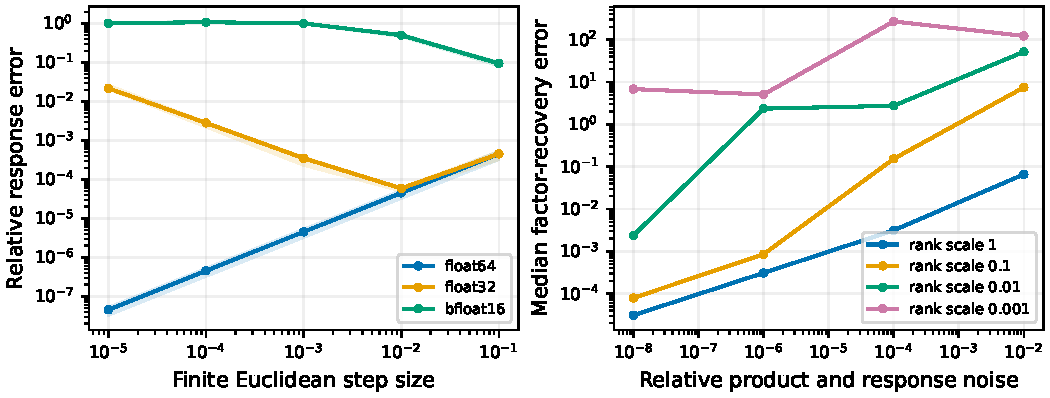
\includegraphics[width=\linewidth]{figures/enhancement_precision.pdf}
\caption{Two numerical limits. Left: finite-step response error at the three
new checkpoints; curves show medians and shading the observed seed range.
Smaller steps reduce FP64 truncation error but amplify low-precision
subtraction error. Right: median factor error over ten synthetic seeds as both
product and response observations are perturbed. The rank scale contracts
the router toward a rank-one uniform matrix; it is not a noise level.
These finite grids are diagnostic rather than worst-case guarantees.}
\label{fig:enhancement-precision}
\end{figure}

\paragraph{Artifacts and scope.}
Versioned protocols and source-bound raw records are supplied under
\texttt{research/} and \texttt{results/enhancement/}, including checkpoints,
seeds and corpus hashes. Each seed's paired bootstrap uses 10,000
resamples of its evaluation blocks; intervals are conditional and do not
substitute for independent training seeds. The new evidence supplements,
rather than overwrites, the original raw records and their negative findings.
